\documentclass{article}
\newcommand\tab[1][1cm]{\hspace*{#1}}
\usepackage{fancyhdr}
\usepackage{enumerate}
\usepackage{enumitem}
\usepackage{amsmath}
\usepackage{amsfonts}
\usepackage{amssymb}
\usepackage{mathtools}
\usepackage{tikz}
\usetikzlibrary{calc}
\newcommand{\N}{\mathbb{N}}
\newcommand{\Z}{\mathbb{Z}}
\DeclarePairedDelimiter\ceil{\lceil}{\rceil}
\DeclarePairedDelimiter\floor{\lfloor}{\rfloor}
%
% Basic Document Settings
%

\topmargin=-0.45in
\evensidemargin=0in
\oddsidemargin=0in
\textwidth=6.5in
\textheight=9.0in
\headsep=0.25in

\linespread{1.1}

\pagestyle{fancy}
\lhead{\hmwkAuthorName}
\rhead{\hmwkClass: \hmwkTitle}
\cfoot{\thepage}

\renewcommand\headrulewidth{0.4pt}
\renewcommand\footrulewidth{0.4pt}

\setlength\parindent{0pt}

\newcommand{\hmwkTitle}{Homework\ \#3}
\newcommand{\hmwkDueDate}{October 30, 2017}
\newcommand{\hmwkClass}{CS 344}
\newcommand{\hmwkClassTime}{Section \#1}
\newcommand{\hmwkClassInstructor}{Professor Bahman Kalantari}
\newcommand{\hmwkAuthorName}{\textbf{Tina Janulis (trj31), Caleb Rodriguez (cjr199), and Rui Zhang (rz187)}}

%
% Title Page
%

\title{
    \vspace{2in}
    \textmd{\textbf{\hmwkClass:\ \hmwkTitle}}\\
    \normalsize\vspace{0.1in}\small{Due\ on\ \hmwkDueDate}\\
    \vspace{0.1in}\large{\textit{\hmwkClassInstructor\ \hmwkClassTime}}
    \vspace{3in}
}

\author{\hmwkAuthorName}
\date{}

\setlength\parskip{\baselineskip}
\begin{document}
\maketitle
\pagebreak

\section*{Problem 1}
\subsection*{Given an undirected  graph G,  describe an algorithm that can check if it is bipartite. A graph is bipartite if its vertices are partitioned into two sets A and B where all the edges are of the form (a,b) with a in A, b in B.}
	You can determine if the graph is bipartite by using BFS. Assign one color (let's say black) to the source vertex, which we will put in set A. Then, color all the neighbors gray, putting them into set B. Color all the neighbors of those neighbors black and put them into set A. When we assign colors, if we find a neighbor with the same color as the current vertex, the graph can't be colored with two vertices. This means that the graph isn't bipartite. A bipartite graph is possible if the graph coloring is possible using two colors such that vertices in a set are colored with the same color.

\section*{Problem 2}
\subsection*{Do a BFS of the undirected graph with the given adjacency list, where starting vertex is x and vertices are placed on queue in alphabetic order. Draw the graph.}
\begin{center}
	\begin{tabular}{c c}
    	Order of Visitation & Queue Contents After Visiting Node\\
        & [x]\\
        x & [t w y]\\
        t & [w y u x]\\
        w & [y u x s]\\
        y & [u x s]\\
        u & [x s]\\
        x & [s]\\
        s & [r]\\
        r & [v]\\
        v & []\\
     	\\
    \end{tabular}
    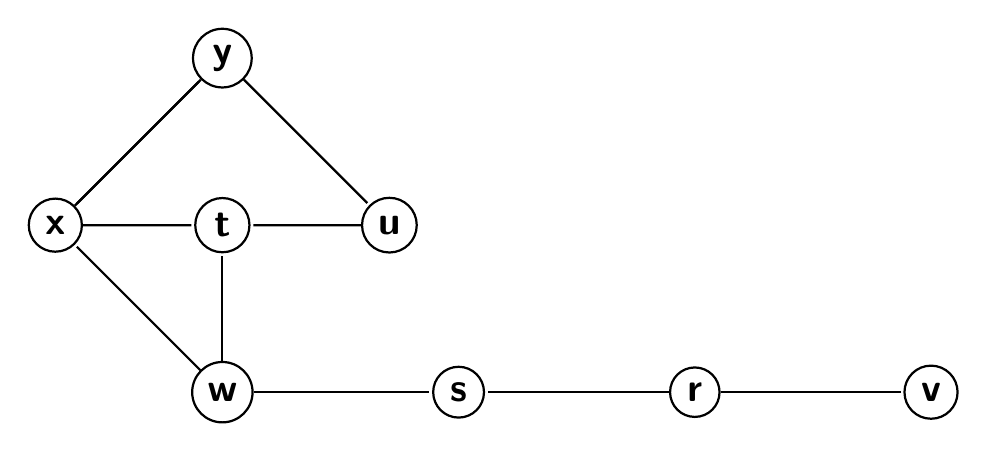
\begin{tikzpicture}[-,shorten >=1pt,auto,node distance=3cm,
                    thick,main node/.style={circle,draw,font=\sffamily\Large\bfseries}]

    \node[main node] (1) {y};
    \node[main node] (2) [below left of=1] {x};
    \node[main node] (3) [below right of=2] {w};
    \node[main node] (4) [below right of=1] {u};
    \node[main node] (5) at ($(2)!0.5!(4)$) {t};
    \node[main node] (6) [right of=3] {s};
    \node[main node] (7) [right of=6] {r};
    \node[main node] (8) [right of=7] {v};

    \path[every node/.style={font=\sffamily\small}]
      (1) edge node [left] {} (2)
      	  edge node [right] {} (4)
      (2) edge node [right] {} (1)
          edge node {} (5)
      (3) edge node [right] {} (2)
      	  edge node {} (5)
          edge node {} (6)
      (4) edge node {} (5)
      (7) edge node {} (6)
      	  edge node {} (8);
 	\end{tikzpicture}
\end{center}
	
\section*{ Problem 3}
	\subsection*{Given a tree $T=(V,E)$ compute its diameter, i.e. the longest path between two vertices. Do BFS at a node s, find the farthest from s to get a vertex, say t. Then do BFS from t to find  the farthest from t.   Prove this gives the diameter of the tree. Diameter of a tree is the longest path in the tree.}
    Assume we have a tree given by $T=(V,E)$.\\
    Assume the algorithm finds a vertex $t$ by performing BFS($s$) on some node $s$.\\
    Then, assume it finds another vertex $r$ by performing BFS($t$) on $t$.\\
    It is clear that $t$ must be a leaf node, since leaf nodes provide the paths with the farthest distance.\\
    It is also clear that $r$ must be a leaf node for the same reason.\\
    Then, d($t,r$) is the diameter of $T$, since it is the longest path between any two leaf nodes.\\
    If the longest path happened to be d($s,t$), then $r=s$.
    

		
\section*{Problem 4}
	\subsection*{Show that in an indirected graph the sum of the degrees of the vertices is twice the number of edges.}
	Any two points on a connected graph is connected by at least one edge. In an undirected graph, for any two vertices $v_1$ and $v_2$ with edges $e_1$, $e_2$, ..., $e_n$ connecting $v_1$ and $v_2$, then for any edge $e_i$ there is of degree two. Therefore, for $n$ edges the number of degrees is $2n$. Assume the base case of where there is only two vertices with a single edge connecting them. Then, the sum of the degrees is 2 and there is only 1 edge and therefore the statement holds. Now, assume that it is true for a graph with $k$ edges and would, therefore have $2k$ degrees. If another edge is added to the graph, then that increases the number of degrees by 2 and therefore, $2k+2 = 2(k+1)$ which shows that the statement holds true for $k$ and $k+1$.

\end{document}
